\section{השירות ותהליך העבודה \en{(Service \& AI Pipeline)}}

\subsection{סקירת התהליך}
התהליך מורכב משישה שלבים. כל שלב מייצר תוצר ביניים הנשמר בארכיון, כך שאפשר לחזור אחורה ולהשוות מקור מול תוצאה.

\begin{figure}[h]
\centering
\begin{english}\begin{tikzpicture}[
  node distance=4mm,
  pstep/.style={draw=mteal,fill=mpaper,rounded corners=3pt,minimum width=21mm,minimum height=12mm,align=center,font=\sffamily\scriptsize,line width=0.8pt},
  hum/.style={pstep,fill=mamber!25,draw=mamber},
  arr/.style={-{Stealth[length=2mm]},line width=0.9pt,color=mtealdark}]
  \node[pstep] (a) {Intake\\ and consent};
  \node[pstep,right=of a] (b) {Scan\\ 1200 dpi};
  \node[pstep,right=of b] (c) {AI\\ restore};
  \node[hum,right=of c] (d) {Human\\ review};
  \node[pstep,right=of d] (e) {Archive\\ and metadata};
  \node[pstep,right=of e] (f) {Delivery};
  \foreach \x/\y in {a/b,b/c,c/d,d/e,e/f} \draw[arr] (\x) -- (\y);
  \draw[arr,dashed,color=msepia] (d.south) -- ++(0,-8mm) -| node[pos=0.25,below,font=\sffamily\tiny]{rework loop} (c.south);
\end{tikzpicture}\end{english}
\caption{תהליך העבודה של \en{Memoria}. השלב הצהוב הוא בקרת אדם; החץ המקווקו מציין חזרה לשחזור מחדש.}
\label{fig:pipeline}
\end{figure}

\subsection{פירוט השלבים}
\paragraph{קליטה והסכמה.} כל הזמנה נפתחת בטופס הסכמה: מי בעל הזכויות בתמונות, האם מותר לעבד תמונות של אנשים מזוהים, ומה מדיניות המחיקה. הלקוח מקבל מספר הזמנה ומדבקת מעקב.

\paragraph{סריקה.} הסריקה מתבצעת ברזולוציה של \num{1200}~\en{dpi} לפחות לתצלומים קטנים, בפורמט \en{TIFF} ללא דחיסה. קובץ המקור נשמר ולעולם אינו נדרס, בהתאם לעיקרון ״המקור הוא קדוש״.

\paragraph{שחזור בסיוע \en{AI}.} השלב משלב שלושה מודלים: הגדלת רזולוציה והסרת רעש \cite{wang2021realesrgan}, שחזור פנים \cite{wang2021gfpgan}, וצביעה אופציונלית \cite{zhang2016colorful}. הצבעים שמוצעים בצביעה הם \emph{פרשנות} ולא עובדה; לכן הם מסומנים כך בארכיון.

\paragraph{בקרת אדם.} מומחה בודק כל תמונה בהגדלה, משווה פנים למקור, ומאשר או מחזיר לעיבוד. זהו שלב הבקרה המרכזי, והוא מאפיין את ההצעה שלנו מול כלי \en{AI} אוטומטיים.

\paragraph{ארכיון ומטא־נתונים.} כל תמונה מתויגת: שמות, מקום, תאריך משוער, מקור, והערות המשפחה. התיעוד נשמר בפורמט פתוח (\en{JSON} ו-\en{CSV}) כדי שלא יהיה קשר ל-\en{Memoria} אם הלקוח יעבור ספק.

\paragraph{מסירה.} הלקוח מקבל קישור מוצפן להורדה, כונן \en{USB} ואלבום מודפס בחבילת \en{Heritage}. הגיבוי נשמר בענן לתקופה שנקבעה בחוזה.

\subsection{מדדי איכות}
\begin{table}[h]
\centering
\caption{מדדי שירות מתוכננים}
\label{tab:sla}
\small
\begin{tabularx}{0.9\textwidth}{>{\bfseries}X l l}
\toprule
\theadrow \thead{מדד} & \thead{יעד} & \thead{שיטת מדידה} \\
\midrule
זמן אספקה, חבילת \en{Basic} & עד \num{5} ימי עבודה & חותמת זמן בקליטה ובמסירה \\
זמן אספקה, חבילת \en{Heritage} & עד \num{15} ימי עבודה & חותמת זמן בקליטה ובמסירה \\
תמונות שהוחזרו לשחזור מחדש & מתחת ל-\num{8}\% & יומן בקרת אדם \\
שביעות רצון לקוח & \num{4.6} מתוך \num{5} ומעלה & סקר לאחר מסירה \\
\bottomrule
\end{tabularx}
\end{table}

\subsection{איך מודדים איכות שחזור}
״נראה טוב״ אינו מדד מספיק לעסק. לכן אנו מגדירים מדדים כמותיים. המדד הנפוץ הוא יחס אות לרעש שיא (\en{PSNR}):
\begin{equation}
  \mathrm{PSNR} \;=\; 10\log_{10}\!\left(\frac{\mathrm{MAX}^2}{\mathrm{MSE}}\right), \qquad
  \mathrm{MSE} = \frac{1}{HW}\sum_{i,j}\bigl(x_{ij}-\hat{x}_{ij}\bigr)^2 ,
\end{equation}
כאשר $x$ התמונה המקורית ו-$\hat{x}$ התמונה המשוחזרת. מדד משלים הוא דמיון מבני (\en{SSIM}), המשווה בהירות, ניגודיות ומבנה:
\begin{equation}
  \mathrm{SSIM}(x,y) \;=\; \frac{(2\mu_x\mu_y + c_1)(2\sigma_{xy} + c_2)}{(\mu_x^2+\mu_y^2 + c_1)(\sigma_x^2+\sigma_y^2 + c_2)} .
\end{equation}
מדדים אלה דורשים תמונת ייחוס נקייה, שאין לנו בתצלומים אמיתיים. לכן ביצענו ניסוי סינתטי: יצרנו בקוד ״תצלום״ מלאכותי, הוספנו רעש וקווי שריטה, והפעלנו מסנן קלאסי פשוט (חציון אופקי וטשטוש ממוצע). זהו קו בסיס ולא המודל שלנו; הוא נועד להדגים כיצד נמדד שיפור. ה-\en{PSNR} עלה מ-\num{\QPsnrBefore}\,\en{dB} ל-\num{\QPsnrAfter}\,\en{dB}, וה-\en{SSIM} הגלובלי מ-\num{\QSsimBefore} ל-\num{\QSsimAfter}.

\begin{figure}[h]
\centering
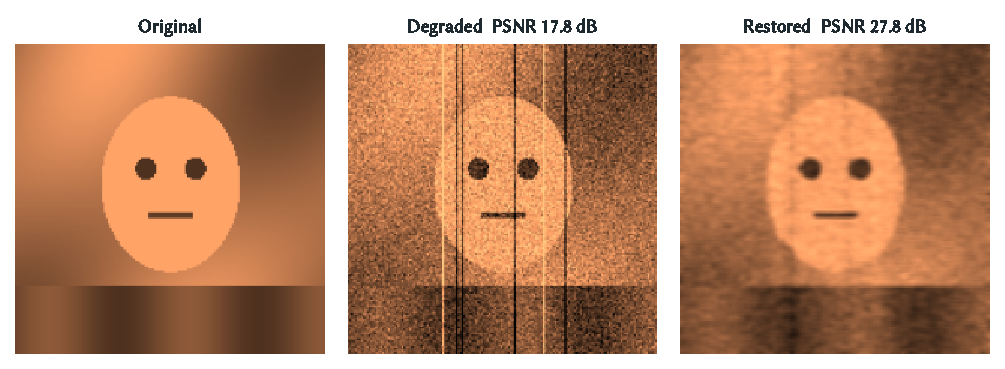
\includegraphics[width=\textwidth]{figures/quality_demo.pdf}
\caption{ניסוי סינתטי: מקור, גרסה פגועה ותוצאת מסנן קלאסי. כל התמונות נוצרו בקוד (\code{code/quality\_demo.py}) ללא תמונות חיצוניות.}
\label{fig:qdemo}
\end{figure}

\begin{figure}[h]
\centering
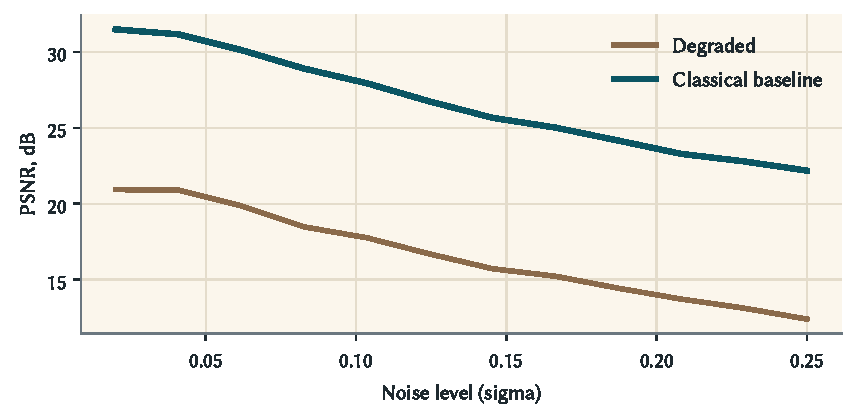
\includegraphics[width=0.72\textwidth]{figures/quality_curve.pdf}
\caption{שיפור \en{PSNR} של קו הבסיס הקלאסי כפונקציה של עוצמת הרעש. ככל שהרעש חזק יותר, השיפור המוחלט קטן, ולכן שחזור קשה דורש מודלים מתקדמים ובקרת אדם.}
\label{fig:qcurve}
\end{figure}

בפועל נשתמש במדדים אלה לבדיקות רגרסיה: אוסף קטן של תמונות בדיקה מדודות מורץ מחדש בכל שדרוג מודל, ושדרוג המוריד את המדדים נדחה. על גבי המדדים הכמותיים מוסיפה בקרת האדם את מה שמספרים אינם רואים: האם הפנים עדיין דומים לאדם האמיתי.
